% 2015四川理 q20 图1：椭圆 x^2/4+y^2/2=1，P(0,1)，过P的动直线l(取k=0.78)交椭圆于A,B
\usetikzlibrary{arrows.meta}
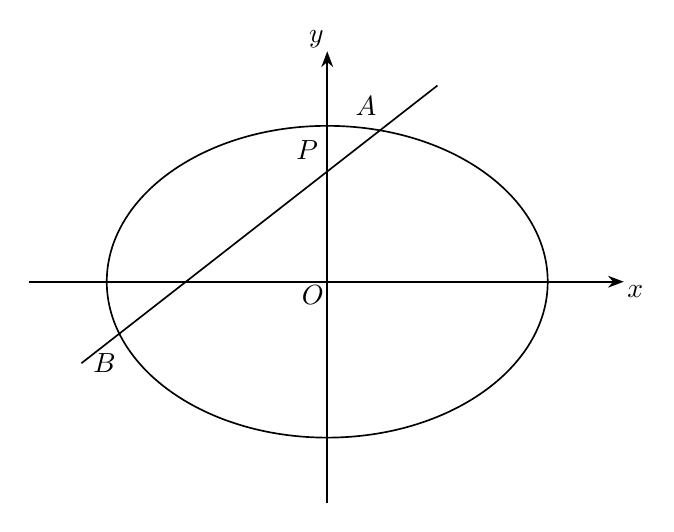
\begin{tikzpicture}[x=1.4cm,y=1.4cm,line width=.6pt,font=\normalsize,>=Stealth]
  \draw[->] (-2.71,0) -- (2.69,0) node[below right,inner sep=1pt] {$x$};
  \draw[->] (0,-2.01) -- (0,2.09) node[above left,inner sep=1pt] {$y$};
  \draw (0,0) ellipse [x radius=2,y radius=1.41421];
  \draw (-2.23000,-0.73940) -- (1.00000,1.78000);
  \node[below left,inner sep=1pt] at (0,0) {$O$};
  \node[above left,inner sep=1pt,xshift=-2pt,yshift=3pt] at (0,1) {$P$};
  \node[above left,inner sep=1pt,yshift=4pt] at (0.47841,1.37316) {$A$};
  \node[anchor=north east,inner sep=1pt,yshift=-6pt] at (-1.88584,-0.47096) {$B$};
\end{tikzpicture}
